\documentclass[12pt]{extarticle}
\def\activityid{F04-M-v2}\usepackage[letterpaper,margin=.65in,top=.60in,bottom=.65in]{geometry}
\usepackage[T1]{fontenc}\usepackage[default]{sourcesanspro}
\usepackage{microtype,tikz,array,tabularx,fancyhdr,amsmath,amssymb}
\usepackage[hidelinks]{hyperref}\usetikzlibrary{calc,arrows.meta}
\setlength{\parindent}{0pt}\setlength{\parskip}{7pt}\setlength{\headheight}{0pt}\setlength{\footskip}{26pt}
\setlength{\emergencystretch}{2em}\pagestyle{fancy}\fancyhf{}\renewcommand{\headrulewidth}{0pt}\renewcommand{\footrulewidth}{.4pt}
\fancyfoot[L]{\scriptsize Bellingham Math Circle / Week 4 / \activityid}\fancyfoot[R]{\scriptsize \thepage}
\definecolor{ink}{gray}{.12}\definecolor{soft}{gray}{.95}\color{ink}
\newcommand{\PageTitle}[2]{{\fontsize{10}{12}\selectfont\bfseries WEEK 4\quad ROUND AND ROUND\hfill #1\par}\vspace{3pt}{\fontsize{26}{29}\selectfont\bfseries #2\par}\vspace{2pt}}
\newcommand{\NameLine}{{\small Name: \rule{2.65in}{.4pt}\hfill Date: \rule{1.35in}{.4pt}\par}\vspace{4pt}}
\newcommand{\Task}[2]{\par\vspace{3pt}{\large\bfseries #1}\par #2\par}
\newcommand{\Subhead}[1]{\par\vspace{3pt}{\large\bfseries #1}\par}
\newcommand{\RuleBox}[1]{\par\begingroup\setlength{\fboxsep}{8pt}\colorbox{soft}{\parbox{\dimexpr\linewidth-16pt\relax}{#1}}\endgroup\par}
\newcommand{\WriteBox}[2]{\par\textbf{#1}\par\vspace{2pt}\begin{tikzpicture}\draw[black!40,line width=.5pt] (0,0) rectangle (\dimexpr\linewidth-.5pt\relax,#2);\end{tikzpicture}\par}
\newcommand{\StudentFooter}{\vfill{\small Try it with objects. Explain by pointing, talking, or drawing.}\par}
\newcommand{\LampRing}[3]{\begin{tikzpicture}[x=1in,y=1in]
\foreach \i in {1,...,#1}{\coordinate (v\i) at ({90-360*(\i-1)/#1}:#2);}
\foreach \i in {1,...,#1}{\pgfmathtruncatemacro{\j}{mod(\i,#1)+1}\draw[thick] (v\i)--node[midway,fill=white,inner sep=2pt,font=\small]{\i\j}(v\j);}
\foreach \i in {1,...,#1}{\node[circle,draw,fill=white,minimum size=.52in,inner sep=0pt,font=\bfseries] at(v\i){\i};}
\foreach \i in {#3}{\node[circle,draw,fill=ink,text=white,minimum size=.52in,inner sep=0pt,font=\bfseries] at(v\i){\i};}
\end{tikzpicture}}
\newcommand{\Lights}[1]{\begin{tikzpicture}[x=.55in,y=.55in,baseline=-.10in]\foreach \v [count=\i] in {#1}{\ifnum\v=1\fill (\i,0) circle(.16in);\else\draw (\i,0) circle(.16in);\fi}\end{tikzpicture}}
\newcommand{\ClockRing}[2]{\begin{tikzpicture}[x=1in,y=1in]\draw[black!30] (0,0) circle(#2);\pgfmathtruncatemacro{\n}{#1-1}\foreach\i in {0,...,\n}{\node[circle,draw,fill=white,minimum size=.35in,inner sep=0pt] at({90-360*\i/#1}:#2){\i};}\draw[-{Stealth},thick] (-.35,.15) arc(155:25:.38);\node[font=\small] at(0,-.18){clockwise};\end{tikzpicture}}
\newcommand{\Key}[2]{\begin{center}\renewcommand{\arraystretch}{1.55}\begin{tabular}{c|*{#1}{c}}in&#2\end{tabular}\end{center}}

\begin{document}

\PageTitle{GRADES 2--3 / 1}{One clue controls the whole code}\NameLine
\RuleBox{Our small alphabet is A, B, C, D, E, F, G, H, I, J. To encode, move the \textbf{same number of places clockwise} for every letter. After J comes A.}
\begin{center}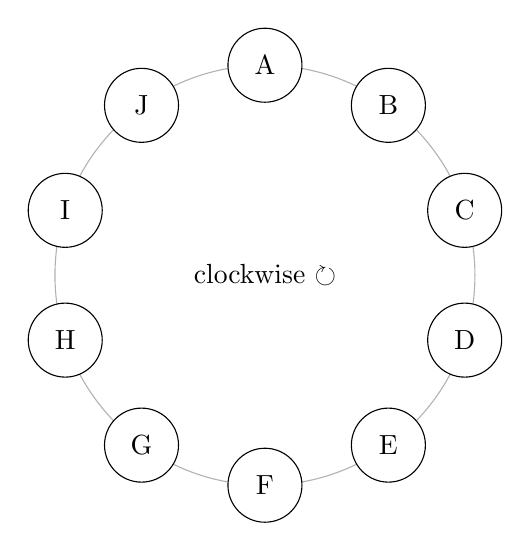
\begin{tikzpicture}[x=1in,y=1in]\draw[black!30](0,0)circle(1.05);\foreach\i/\l in {0/A,1/B,2/C,3/D,4/E,5/F,6/G,7/H,8/I,9/J}{\node[circle,draw,fill=white,minimum size=.37in]at({90-36*\i}:1.05){\l};}\node at(0,0){clockwise $\circlearrowright$};\end{tikzpicture}\end{center}
\Task{1. Recover the key.}{You learn that message A becomes code D. Decode \textbf{GDG}. Then encode \textbf{BAG}. Check by reversing your moves.}
\WriteBox{My shift, decoded message, and new code:}{.8in}
\Task{2. A clue that cannot fit.}{Someone also claims B becomes F under that same key. Could both clues be true? Show why on the ring.}
\WriteBox{My reason:}{.7in}
\StudentFooter
\newpage
\PageTitle{GRADES 2--3 / 2}{A code that skips places}
\Task{3. Repeat a two-step code.}{Start at A. Take two clockwise steps each turn. Write each \textbf{landing} until you first return to A. Do not include skipped-over letters. Which letters never appear?}
\WriteBox{My two-step route and the missing letters:}{.85in}
\Task{4. Repeat a three-step code.}{Start at A again. Take three steps each turn. Does this rule visit every letter before returning? Give the whole route so someone else can check.}
\WriteBox{My three-step route:}{.85in}
\Task{5. Explain the split.}{Start the two-step rule at B instead. How do its landings relate to your route from A? Why can the A-route never jump into the B-route?}
\WriteBox{Two loops, and why they cannot meet:}{1.0in}
\textbf{Go further:} Which step sizes from 1 to 9 visit all ten letters? Can a two-step code still be \emph{decoded} even though one repeated route skips letters?
\StudentFooter

\end{document}
